\section{Function Component} \label{sc:function_component}
Having added new attributes, classes, and structures to the class diagram through the model component, the functions from the function list can be implemented as well. Some of the functions should be implemented in the classes directly, others should be places in the function component. The following section contains additions to the original function list, the arguments for these additions, decisions about implementations of these, and the final function component design.

\subsection{Additions to the function list}
The function list has been constructed based on the original class diagram, but does not accommodate the new additions from the model component. To support the new classes, the following functions have been added:

\begin{table}[H]
\centering
    \begin{tabular}{c|l|l|l}
        \textbf{Nr.} & \textbf{Function name} & \textbf{Complexity} & \textbf{Function type}\\
        \hline
        1 & Get asset by id & Simple & Read\\
        \hline
        2 & Get department by id & Simple & Read\\
        \hline
        3 & Get tag by id & Simple & Read\\
        \hline
        4 & Search for tag & Medium & Compute/Read\\
        \hline
        5 & Add field to asset/tag & Medium & Update\\
        \hline
    \end{tabular}
\end{table}

Function 1-3 are added to return the objects from the model to the application domain. The \textit{get asset by id} function replaces the \textit{view asset} function, as they serve the same purpose.\\
Function 10 handles the tagging of an asset by creating the tag relation between the asset and the tag to be attached.\\
Function 4 makes it possible to search for a tag, as it was previous possible to search for an asset.\\
Function 5 makes it possible to add a field to an asset or a tag.
\par
The updated function list has then been implemented in the component deign. Classes, attributes, and structures have been added simultaneously in this section, as they often can not exist alone.

\subsection{Design}
The following includes examinations of the functions and design decisions about how they should be incorporated in the component design.

\subsubsection{Maintaining model}
All the add, remove, update, and get by id functions are used by the employee with admin status. These functions should be handled similarly for assets, departments, and tags, and therefore they will all be grouped into a strategy. A thorough look at these functions and the structure will show that this pattern is actually a repository pattern. Hence an intuitive name of the overall strategy is \textit{Repository}, and the strategy is abstract, as every concrete strategy will inherit the functions. The concrete strategies handle the assets, departments, and tags respectively and has been named: \textit{AssetRepository}, \textit{DepartmentRepository}, and \textit{TagRepository}. These control the maintenance of the data for their designated classes in the model.
\par
As mentioned, these concrete strategies have operations for adding, removing, and updating, which all take an object of the designated class, and an operation for getting an object by id, which takes the id of the wanted object. The structure has been placed in the function component, as it does not belong to a specific class in the model component but will be used by admin employees.
\begin{figure}[H]
    \centering
    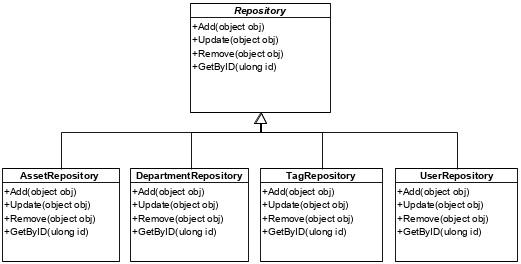
\includegraphics[width=0.8\textwidth]{figures/FunctionComponent/Repository_pattern.png}
    \caption{The repository pattern for maintaining data in the model}
    \label{fig:RepositoryPattern}
\end{figure}

\subsubsection{Attach/detach tag}
The operations of attaching or detaching an asset is called by an admin employee and involves the \textit{Tag} and \textit{Asset} classes. The functions create or delete an instance of the \textit{Asset-tag relation} class containing the involved asset and tag. The operations should be added to a class in the function component, as the admin employee does not carry out the operations. They have been placed in the \textit{AssetRepository} class, as it handles the assets. Placing them directly on the \textit{Asset} class however, would give the class responsibility of an operation in which it participate solely in as an object. For clarity, the operations have been named \textit{AttachTag} and \textit{DetachTag}.\\
Both operations take two parameter, an asset, and a list of tags to be attached to the asset.
\begin{figure}[H]
    \centering
    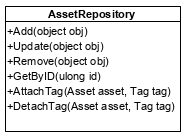
\includegraphics[width=0.3\textwidth]{figures/FunctionComponent/AttachTag.png}
    \caption{The \textit{AssetRepository} class with the \textit{AttachTag} and \textit{DetachTag} operations}
    \label{fig:AttachDetachTag}
\end{figure}

\subsubsection{Search for asset or tag}
\todo[]{Kommer vi til at kunne søge i comments og users skal dette også beskrives hvis det bliver en realitet.}
The 'search for asset' function lets the employee search through the assets in the system and returns the assets that comply with the search query. Multiple assets are handled and therefore it would not be intuitive to add it as an operation on the asset class. It is called by the employee, but the employee does not stand with the responsibility of searching through the assets, so the function has been placed as an operation in the function component.\\
The function 'search for tag' goes through the same process and both functions have the same structure. The search is carried out on the elements in the database and therefore they fit well into the concrete strategies of the \textit{Repository} strategy.
\begin{figure}[H]
    \centering
    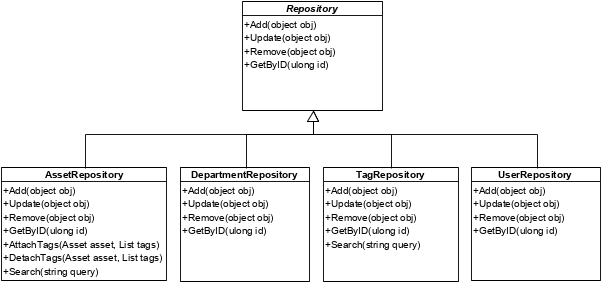
\includegraphics[width=0.8\textwidth]{figures/FunctionComponent/Repository_pattern_with_search.png}
    \caption{The repository pattern with the search operations for assets and tags}
    \label{fig:RepositoryPatternWithSearch}
\end{figure}

\subsubsection{Comment asset}
Commenting an asset adds a comment to the asset. It is desired that the comments can be retrieved and shown without knowledge about the asset to which it belongs. The reason for this is that the newest comments to be shown on the home page of all admins, to give an overview about newest changes and problems. Therefore the comments will not be placed directly on the asset, but will be stored separately and contain a connection to the asset.\\
Because of this, the comment will need the function function add, remove, update, and get by id and can therefore be seen as another concrete strategy of the \textit{Repository}.
\begin{figure}[H]
    \centering
    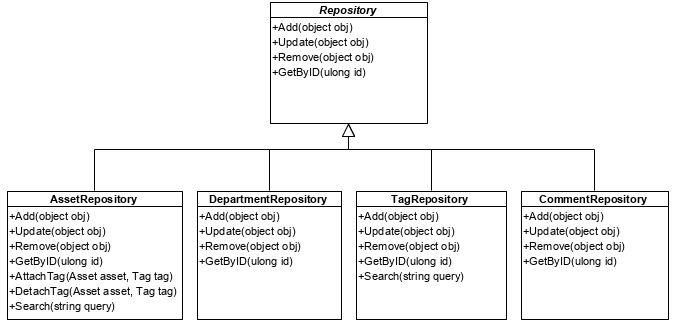
\includegraphics[width=0.9\textwidth]{figures/FunctionComponent/CommentRepository.png}
    \caption{The repository pattern with the \textit{CommentRepository}}
    \label{fig:RepositoryPatternWithCommentRepository}
\end{figure}

% \subsubsection{View asset}
% Viewing an asset means being send to a page with the asset illustrated with relevant information. The function retrieves the given asset from the database. As the function is simply reading form the database, it fits well into the \textit{MaintainModelAssets} class in the function component.
% \todo[inline]{Insert structure diagram with the new operations for asset}

\subsubsection{Authenticate user \& Check access level}
The authentication and access level check are both functions that has been handled by the \textit{Employee} class. As the employee should not do these things itself, the functions have been moved to the function component and implemented as operations in a class called \textit{Session}. They have been renamed to \textit{Authenticated} and \textit{IsAdmin} and return rather the employee currently logged into the system is authenticated and has admin authority respectively. This makes both the \textit{Employee} and \textit{Admin} classes obsolete. This class also contains the attributes \textit{Username} and \textit{Domain}, to make sure that these information about the employee currently logged in are available to the system.
\begin{figure}[H]
    \centering
    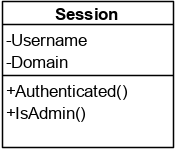
\includegraphics[width=0.3\textwidth]{figures/FunctionComponent/Session.png}
    \caption{The \textit{Session} class}
    \label{fig:session_class}
\end{figure}

\subsubsection{Add field to asset/tag}
Adding a field to either an asset or a tag will create a field directly on the asset or tag. The fields do not have their separate place in the system, as they are not relevant without either the asset or the tag, to which it belongs. Therefore the function has been implemented in the function component as an operation in a class called \textit{FieldController}.\\
The operation takes in two paramters. The object to which the field should be attached to, written as the type \textit{FieldContainable}, as it can be either an asset or a tag, and the \textit{Field} that should be attached.
\begin{figure}[H]
    \centering
    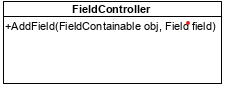
\includegraphics[width=0.6\textwidth]{figures/FunctionComponent/FieldController.png}
    \caption{The \textit{FieldController} class}
    \label{fig:FieldController}
\end{figure}

\subsubsection{Export report}
The only class needing access to this function is the \textit{Employee} class. The function is not relevant for any other class, but the responsibility for executing the operation does not lie with the \textit{Employee} class itself. Therefore, the operation has been moved into a class in the function component named \textit{ExportHandler}.
\begin{figure}[H]
    \centering
    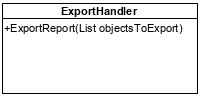
\includegraphics[width=0.4\textwidth]{figures/FunctionComponent/ExportHandler.png}
    \caption{The \textit{ExportHandler} class}
    \label{fig:ExportHandler}
\end{figure}

\subsection{Specification of complex functions}
The complex functions have been depicted with further descriptions, to ease the understanding process of them. Some of the complex function are trivial and therefore have not been described in further detail. This includes the search assets and tags operations.
% This includes the adding and removing of assets, departments, and tags, updating these as it is simply changing the value of attributes, and searching through the sets.
\par
This leaves the Export report function to be described in further detail.
\begin{table}[H]
    \centering
    \hrule
    \begin{tabular}{p{5cm} p{8cm}}
    \\
         \textbf{Name} & Export report \\\\
         \textbf{Category} & Passive read\\\\
         \textbf{Purpose} & Creates a CSV-file and saves it on the users computer.\\\\
         \textbf{Input} data & Collection of elements to be exported in the CSV-file.\\\\
         \parboxc{t}{1ex}{\textbf{Conditions}} & The user has selected one or more elements to be exported.\newline A location on the users computer to store the file.\\\\
         \textbf{Effect} & A CSV-file containing the collection of elements.\\\\
         \textbf{Algorithm} & -\\\\
         \textbf{Data structures} & Enumerable list\\\\
         \textbf{Placement} & ExportHandler\\\\
         \textbf{Involved objects} & Asset\\\\
         \textbf{Triggering events} & export report\\\\
    \end{tabular}
    \hrule
    \caption{Specification of the \textit{Export report} operation}
    \label{tab:complex_func_description_export_report}
\end{table}
\par
The overall behaviour of the system is pretty simple, as it only has the state \textit{active}. Therefore, a diagram of this behaviour is trivial and has not been included here.
\par
The function component has then been constructed and is illustrated below in \autoref{fig:FunctionComponent}.
\begin{figure}[H]
    \centering
    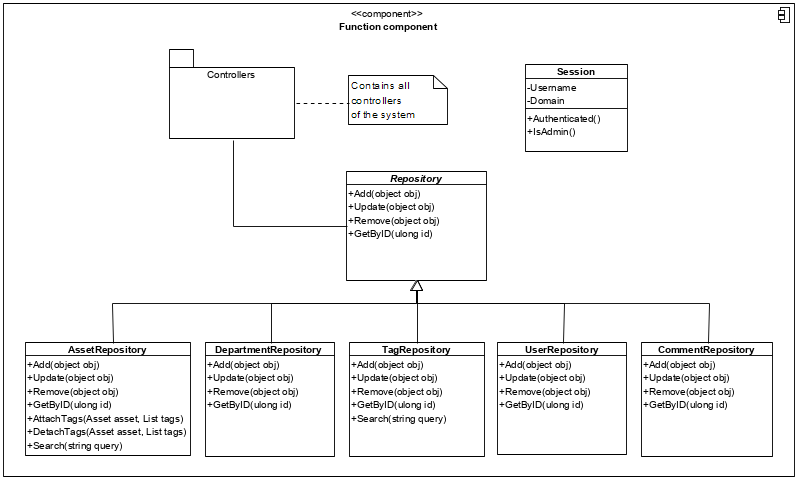
\includegraphics[width=0.8\textwidth]{figures/FunctionComponent/FunctionComponent.png}
    \caption{Illustration of the function component of the system}
    \label{fig:FunctionComponent}
\end{figure}